\section{Engine and Transmission Module}

The engine and transmission module implements the design specified in Sec.\ \ref{sec:engine_transmission_design}. Figure \ref{fig:engine_transmission_pcb} shows a photo of the module after being populated and debugged.

\begin{figure}[H]
\centering
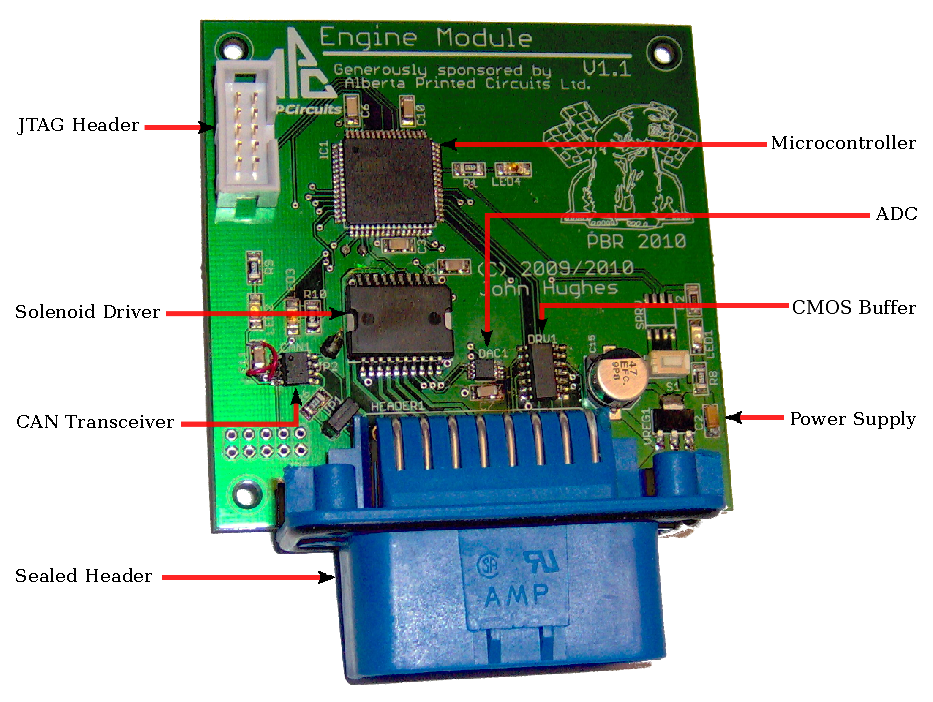
\includegraphics[scale=1]{implementation/figures/engine_transmission_pcb}
\caption{Photograph of the populated engine and transmission module PCB.}
\label{fig:engine_transmission_pcb}
\end{figure}

\subsection{Hardware}
\nomenclature{SPI}{Serial Peripheral Interface}
\nomenclature{CMOS}{Complimentary Metal-Oxide-Semiconductor}
\nomenclature{DAC}{Digital-to-Analog Converter}

In addition to the base system hardware common to all modules described in Sec.\ \ref{sec:base_system_hardware}, three additional hardware components are required. A single \emph{serial peripheral interface} (SPI) capable \emph{low-side solenoid driver} implements the solenoid driver requirement laid out in Sec. \ref{sec:design_engine_transmission_hardware}. A \emph{complimentary metal-oxide-semiconductor} (CMOS) buffer chip is used to interface the discrete pins on the ECU (as described in Sec.\ \ref{sec:ecu_background_discrete_inputs}). An SPI capable \emph{digital-to-analog converter} (DAC) provides the \unit{0-5}{\volt} output signal required to set the traction control slip percentage.

Figure \ref{fig:engine_system_overview} shows a block-level diagram of the hardware implementation of the engine and transmission module, including the specific components chosen for the implementation. A list of the components additional to the base system hardware can be found in Table \ref{tab:engine_transmission_module_components}.

\begin{figure}[H]
\centering
\begin{tikzpicture}[auto, node distance=3.5cm, draw=black!70, >=stealth']
  \node [block, name=at90] {AT90CAN};
  \node [block, name=dac, left of=at90] {TLV5623 DAC};
  \node [block, name=driver, right of=at90] {L9822E Solenoid Driver};
  \node [block, name=can, below of=at90, above=0.5cm] {MCP2551 CAN Transceiver};
  \node [block, name=buf, left of=can] {74LVC07 Buffer};

  \node [block, name=ecu, rotate=90, minimum width=8em] at ($(dac.west)!0.5!(buf.west)+(-1.25cm,0)$) {ECU};
  \node [block, name=solenoids, right of=driver, left=-0.75cm] {Solenoids};
  \node [block, name=feedback, below of=solenoids, above=0.75cm, text width=2.2cm, inner sep=0.05cm] {Position Transducers};

  \path (at90.north)+(0.0,+0.4) node (title) {Engine Module};

  \begin{pgfonlayer}{background}
    \path (dac.north west)+(-0.3,0.7) node (a) {};
    \path (can.south -| driver.east)+(+0.3,-0.2) node (b) {};
    \path[module] (a) rectangle (b);
  \end{pgfonlayer}

  \node [bus, name=can1, below of=can, label=below:CAN Bus, above=2.0cm] {CAN Bus};
  \node [bus, name=can2, left of=can1] {};
  \node [bus, name=can3, right of=can1] {};

  \draw [-, line width=3pt] (can) -- (can1);
  \draw [-, line width=3pt] (can1) -- (can2);
  \draw [-, line width=3pt] (can1) -- (can3);

  \draw [->, thick] (driver) -- (solenoids);

  \draw [->, thick] (at90) -- node[above] {SPI} (driver);
  \draw [<->, thick] (at90) -- (can);
  \draw [->, thick] (at90) -- node[above] {SPI} (dac);
  \draw [->, thick] ($(at90.west)+(0,-0.3)$) to[myncbar, arm=0.5cm, angle=180] (buf);
  \draw [<-, thick] ($(at90.east)+(0,-0.3)$) to[myncbar, arm=0.5cm] (feedback);

  \draw [->, thick] (dac.west) to[myncbar, arm=0.2cm, angle=180] ($(ecu.south)+(0,0.5)$);
  \draw [->, thick] (buf.west) to[myncbar, arm=0.2cm, angle=180] ($(ecu.south)+(0,-0.5)$);
% 
% 
%   \draw [-, line width=2pt] (can1) -- (can2);
%   \draw [-, line width=2pt] (can2) -- node[rotate=90, above] {CAN Bus} (can3);
%   \draw [-, line width=2pt] (can3) -- (can4);
% 
%   \node [bus, above of=can1, below=1cm] (tip1) {};
%   \node [bus, below of=can4, above=1cm] (tip2) {};
%   \draw [-, densely dashed, line width=2pt] (can1) -- (tip1);
%   \draw [-, densely dashed, line width=2pt] (can4) -- (tip2);
% 
%   \node [block, right of=can2, right, text width=8em] (engine) {Engine Module};
%   \node [block, right of=can3, right, text width=8em] (ecu) {ECU};
% 
%   \node [block, right of=engine, right, text width=8em] (starter) {Starter System};
%   \node [block, right of=ecu, right, text width=8em] (intake) {Intake System};
%   \node [block, above of=starter, text width=8em] (transmission) {Transmission System};
% 
%   \draw [<->] (engine) -- (ecu);
%   \draw [<->] (engine.south east) -- (intake.north west);
%   \draw [<->] (engine) -- (starter);
%   \draw [<->] (engine.north east) -- (transmission.south west);
% 
%   \draw [<->, line width=2pt] (can2) -- (engine);
%   \draw [<->, line width=2pt] (can3) -- (ecu);
\end{tikzpicture}
\caption{Overview of the engine and transmission module hardware.}
\label{fig:engine_system_overview}
\end{figure}

\begin{table}[H]
  \caption{List of components used by the engine and transmission module.}
  \centering
  \begin{tabular}{|c|c|c|}
    \hline 
    Part & Manufacturer & Part Number\tabularnewline 
    \hline \hline
    Solenoid Driver & ST Microelectronics & L9822E \tabularnewline
    \hline
    Digital to Analogue Converter & Texas Instruments & TLV5623C \tabularnewline
    \hline
    Hex CMOS Buffer & Texas Instruments & 74LVC07A \tabularnewline
    \hline
  \end{tabular}
  \label{tab:engine_transmission_module_components}
\end{table}

\subsubsection{High Current Solenoid Driver}

An 8-way solenoid driver component from ST Microelectronics called the LT9822E is used to energize the multiple solenoids of the electro-pneumatic system. The LT9822E provides a simple SPI interface and also has built-in clamping diodes to eliminate the effects of fly-back. This driver reduces the complexity of the output stage of the circuit by eliminating the need for multiple high-current transistors.

\subsubsection{CMOS Buffer}

A standard 74LVC07A CMOS buffer chip is used to buffer the GPIO lines on the microprocessor and the discrete input pins on the ECU. The buffer isolates the two systems and protects the micro-controller from risk of damage via shock.

\subsubsection{Traction Control Analog Output}

The TLV5623C SPI-interfaced DAC from Texas Instruments generates the \unit{0-5}{\volt} analog signal for the ECU's traction slip percent input (described in Sec. \ref{sec:ECU}.) The TLV5623 outputs a \unit{0-5}{\volt} analog signal that varies with the digital input. The output voltage from the DAC is determined by the following equation: \cite{TLV5623}

\begin{equation}
V_{out}^{DAC}=2\cdot{V_{ref}^{DAC}}\,\frac{Code}{2^{n}}\,\volt
\end{equation}

where $V_{ref}$ is the reference voltage input to the chip, $n=8$, and $Code$ is the digital input value sent over SPI ranging from $0$ to $2^{n-1}$. Since we want to output $\unit{5}{\volt}$ at full-scale input,

\begin{equation}
2\cdot{V_{ref}^{DAC}}\,\frac{2^{7}}{2^{8}}=V_{ref}^{DAC}=\unit{5}{\volt}
\end{equation}.

The $V_{ref}$ pin on the DAC was therefore connected to VCC.

\subsection{Software}

The low-level portions of the engine and transmission module software exist, but have yet to be integrated into the high-level managers described in the design. Each of those integral portions are described below.

\subsubsection{Event Scheduler}

The event scheduler allows the module software to request that a particular function be called at some particular time in the future. It works by allocating an array of \emph{tasks} that describe:

\begin{itemize}
	\item the time (in milliseconds) to execute the task;
	\item the function to be executed; and
	\item arguments to the function.
\end{itemize}

Tasks flow from the scheduler into a \emph{task queue}, where they wait until they become current. They are then moved into a \emph{pending queue}, where they wait for \emph{task execution} by the module software. A maximum of fifty tasks can be scheduled or pending at any given time. Task structures are pre-allocated to avoid the use of dynamic memory allocation techniques.

\paragraph{Task Queue} The module software can request a new task be scheduled, and specifies the execution time as an offset from the current system time. The scheduler then calculates the actual time of the task and slots the task into the task queue. This queue is indexed by execution time, with the earliest time at the head.

\nomenclature{FIFO}{First-In First-Out}

\paragraph{Pending Queue}  The scheduler interrupts the program every millisecond to increment it's internal clock. Every interrupt, it checks to see if any events are pending execution. If so, they are appended to the pending queue, which is a standard \emph{first-in first-out} (FIFO) queue. 

\paragraph{Task Execution} The module software may request the next pending task from the scheduler. If there are tasks in the pending queue, the head of the queue is passed to the software for execution, and the head is updated to the next pending task. If no tasks are pending, the module software is notified. This scheme allows the module software to execute pending tasks as processing time becomes available.

\subsubsection{PWM Generator}

The PWM generator is capable of outputting two synchronized PWM signals, $PWM_A$ and $PWM_B$, to the L9822E driver chip. A timer peripheral on the micro-controller is configured to generate periodic interrupts. Different combinations of the PWM duty cycles can be modulated within the interrupt cycle, as described below.

\paragraph{Interrupt} The \unit{32}{\kilo\hertz} external crystal was used as the input to an 8-bit timer peripheral on the micro-controller. The input to the timer was first scaled by 8 to provided a timebase $TB$:

\begin{equation}
TB=\frac{32.768\, kHz}{8}=4.096\, kHz
\end{equation}

The timebase period is then given by:

\begin{equation}
\frac{1}{TB}\approx244\,\mu{S}
\end{equation}

We then define a constant scaling factor in software for the PWM generator:

\begin{equation}
{PWM\_SCALE}=\frac{1}{TB\cdot{f_{PWM}}}\approx205,
\end{equation}

In this case, $f_{PWM}$ is the PWM frequency desired, in our case \unit{20}{\hertz}.

By loading the timers \emph{compare register} with with a value scaled by ${PWM\_SCALE}$, we can cause the timer to generate an interrupt precisely when a level change in the PWM is required.

\paragraph{Algorithm}

Figure \ref{fig:pwm_cases} shows 8 different combinations of the duty cycles of two synchronized PWM channels. Since the waveforms are synchronized, there are only two cases where three transitions per period are required: one at the beginning, and two for falling edges of both channels (corresponding to \ref{fig:pwm_cases_1} and \ref{fig:pwm_cases_2}.) This happens when both channels have $0\%<Duty<100\%$. Two cases are also visible where no transitions are required, shown in \ref{fig:pwm_cases_7} and \ref{fig:pwm_cases_8}.

An efficient generating routine was constructed to effect the level transitions by sending new data to the solenoid driver, and to reset the timer to interrupt at the next transition. For the two cases requiring three transitions per period, the timer interrupts three times per period. For the two cases where both channels have duty cycle between 0 and 100\%, the routine still interrupts once to allow for a change in duty cycle. For the rest of the cases described, the timer only interrupts twice per PWM period.

\begin{figure}[ht]
  \centering
  \subfigure[Case 1]
  {
    \label{fig:pwm_cases_1}
    \begin{tikztimingtable}
      $PWM_A$		& G 4H 4L \\
      $PWM_B$		& G 2H 6L \\
    \end{tikztimingtable}
  }
  \subfigure[Case 2]
  {
  \label{fig:pwm_cases_2}
  \begin{tikztimingtable}
    $PWM_A$		& G 4H 4L \\
    $PWM_B$		& G 6H 2L \\
  \end{tikztimingtable}
  }
  \subfigure[Case 3]
  {
  \label{fig:pwm_cases_3}
  \begin{tikztimingtable}
    $PWM_A$		& G 4H 4L \\
    $PWM_B$		& 8L \\
  \end{tikztimingtable}
  }
  \subfigure[Case 4]
  {
  \label{fig:pwm_cases_4}
  \begin{tikztimingtable}
    $PWM_A$		& G 4H 4L \\
    $PWM_B$		& G 8H G \\
  \end{tikztimingtable}
  }
  \subfigure[Case 5]
  {
  \label{fig:pwm_cases_5}
  \begin{tikztimingtable}
    $PWM_A$		& G 8H G \\
    $PWM_B$		& G 4H 4L \\
  \end{tikztimingtable}
  }
  \subfigure[Case 6]
  {
  \label{fig:pwm_cases_6}
  \begin{tikztimingtable}
    $PWM_A$		& 8L \\
    $PWM_B$		& G 4H 4L \\
  \end{tikztimingtable}
  }
  \subfigure[Case 7]
  {
  \label{fig:pwm_cases_7}
  \begin{tikztimingtable}
    $PWM_A$		& 8L \\
    $PWM_B$		& 8L \\
  \end{tikztimingtable}
  }
  \subfigure[Case 8]
  {
  \label{fig:pwm_cases_8}
  \begin{tikztimingtable}
    $PWM_A$		& G 8H G \\
    $PWM_B$		& G 8H G \\
  \end{tikztimingtable}
  }
  \caption{PWM Cases (1 period shown).}
  \label{fig:pwm_cases}
\end{figure}

\subsubsection{Solenoid Driver}

The low-level solenoid driver uses the SPI library described in Sec. \ref{sec:impl_spi_driver} to communicate with the LT9822E solenoid driver IC. The LT9822E uses a simple one-byte command format: each bit represents one of the eight solenoid outputs. A zero bit turns the solenoid off, while a one bit turns the solenoid on. 

The solenoid driver maintains the current state of the solenoids and allows the module software to toggle the solenoid outputs individually. When toggling a solenoid, the original solenoid state undergoes an ``exclusive-or'' with the bit position of the desired solenoid. This new command byte is then pushed out over the SPI interface, and saved for the next transition.
